\section{Introduction}\label{sec:introduction}
    % \todo[inline]{Here goes short introduction with mention that this is a work about \acf{tool}}
    The idea to create a simulation and control toolkit for small satellite projects was a byproduct of work done on IRISC project by the author of this thesis. IRISC, or "InfraRed Imaging of astronomical targets with a Stabilized Camera", was a project realized as a part of \ac{bexus} programme. The goal of the IRISC experiment was to obtain images in the \ac{nir} spectrum from astronomical targets. Possible targets included the Andromeda Galaxy, Pinwheel Galaxy, Iris Nebula, Eagle Nebula and Starfish Cluster. The images were obtained using a highly stabilized telescope with NIR camera mounted on a \ac{bexus} balloon. Author's responsibility covered the design of the control subsystem of the experiment. The stabilization was achieved by a gimbal-like system, to obtain high quality images while being on a moving platform\cite{irisc-sed}. While the design of the control system was not innovative, nevertheless it was a complicated task for a student with no previous practical experience in that field. This has proven to be especially challenging during early stages of experiment design.

    The process of effective space-related project management - from the conception of the idea, through production, to disposal - features high costs and often various unpredictable risks. Due to this, a project life cycle is usually divided into distinct phases, allowing for introduction of conducting product reviews within rigid time-frames. An example of such a workflow, adopted by most major agencies such as ESA\cite{managementecss} and NASA\cite{kapurch2010nasa}, is a division of the project life cycle into phases, as it can be seen on \autoref{fig:phases}. While the design of a project is often an iterative process, the phases and reviews that conclude them exist as a checkpoints, after which the design of the project is to be unchanged, on a level of details progressing as phases do. For example, as one can see, Phase B is usually ended by the \ac{pdr}. In the case of a spacecraft, for the \ac{pdr}, a major architecture parameters have to be defined, such as volume and weight ramifications, top-level designs of solutions for major requirements have to be presented - for a practical example: for high-resolution Earth observation mission the type of the actuators which fulfills precision requirements has to be chosen.

    \begin{figure}[H]
        \centering
        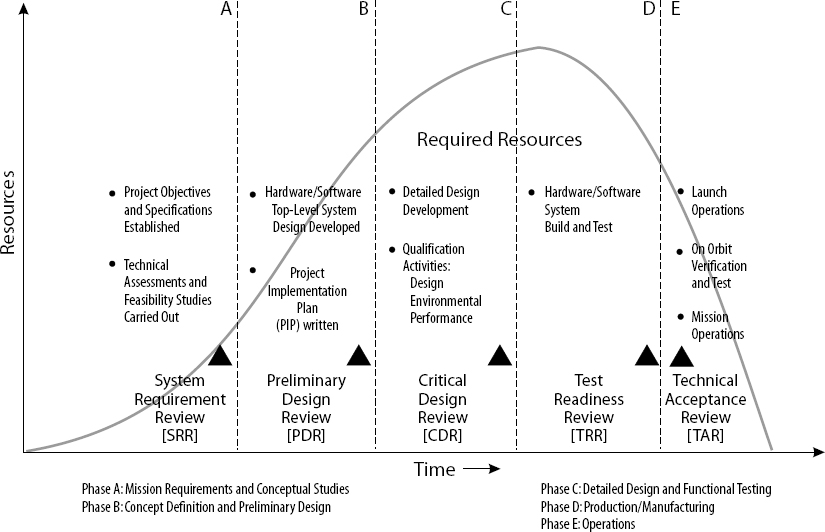
\includegraphics[width=1\textwidth]{1-introduction/phases}
        \caption{Typical space project phases and its life cycle\cite{nguyen2000effective}}
        \label{fig:phases}
    \end{figure}

    Taking the experience of how challenging and time-consuming was the process of learning how to produce a reliable simulation of IRISC control system and the knowledge of significance of preliminary design, author decided to produce and publish a simulation, which would be useful for purposes of initial spacecraft design and for beginner engineers to learn how to build a reliable simulation. 
    

\subsection{Scope}
    The thesis covers the process of development of the toolbox for rapid prototyping of satellite's control systems. \autoref{sec:introduction} describes the aim of this work and discusses the topic of prototyping tools. \autoref{sec:toolbox} goes into detail about the architecture of \ac{tool}, its features and methods of implementation. Also here there are described the ways of connecting \ac{tool} with various visualization tools. \autoref{sec:documentation} explains the documentation and usage of \ac{tool}, while in \autoref{sec:examples} there are examples showing how the toolbox can be used in real life applications. Finally, \autoref{sec:conclusions} discusses the conclusions from the development process and the possibilities for improvements of \ac{tool}.

\subsection{Aim}\label{sec:aim}
    The aim of this thesis work is to build and provide a ready to use open source product - a toolbox for small and low budget satellite projects.  The toolbox features allow for a initial design of spacecraft's \ac{adcs}, which means that they allow for, i.a. simulation of spacecraft orbit, testing the feasibility of various actuation methods and testing the effectiveness of different control algorithms in given use cases. That software would then allow smaller and inexperienced teams of spacecraft designers to better prepare for design milestones like \ac{pdr}, when there is not enough time to create a full simulation of their spacecraft \ac{adcs} subsystems. Besides the toolbox being a tool for practical use, the thesis also serves as as a review of available solutions, so it can be used by future control engineers as a learning material. The idea is, that some parts of the proposed model could be removed from the model as the students, for the learning purposes, would be tasked with designing a substitution.

    For the purposes of later evaluation of how the solutions proposed in this thesis fulfil the goals stated in the preceding paragraph, a following list of objectives was compiled:

    \begin{itemize}
        \item \textbf{Conduct a review of existing tools for preliminary spacecraft design}, focusing on mission planning and \ac{aocs} subsystem;
        \item \textbf{Create a spacecraft dynamics and \ac{aocs} model}, to be used with minimal set-up;
        \item \textbf{Assemble a library of models}, to be used by other beginner control engineers;
        \item \textbf{Provide a documentation of the toolbox}, explaining not only the purpose and  operating principles of individual parts, but the process of using the toolbox to conduct a preliminary design of spacecraft \ac{aocs} subsystem;
        \item \textbf{Share the toolbox to be available online}, with principles of open-source software in mind.
    \end{itemize}

    Furthermore, the objectives that are set for the design of the toolbox itself are described in Chapter \ref{toolbox:objectives}.

\subsection{Digital prototyping tools}
% \todo[inline]{refer to CAE software}
    \dots\textit{description of CAD software}\dots

\subsection{Already existing tools}
    % ... This is to show that, while the toolbox for \ac{adcs} prototyping or development is not an innovative idea, but since some existing solutions are not best fit for the job of rapid prototyping and others are unavailable or paid, there is a need for a new, open-source one.

    The idea for a toolbox allowing for spacecraft mission design and \ac{aocs} simulation is not a new one. There are various solutions available, ranging from very robust commercial software packages to open-source implementations of individual features for use as a part of MATLAB framework.

    The aim of this section is to prove that, while the solutions for spacecraft prototyping are available, there is still a need for open-source, easy-to-sue and modify toolbox. Further below is a compiled list of selected software solutions that fit the most objectives stated in \autoref{sec:aim}, with included explanation what they are lacking that discussed toolbox should have.
 
    % \todo{Should I put "advantages" and "disadvantages" here at the end of every point?}

    \subsubsection{MATLAB CubeSat Simulation Library}
        % \todo{how to write that it was considered to expand this rather than develop own toolbox}
        CubeSat Simulation Library is a part of Aerospace Blocks created by MathWorks Aerospace Products Team. Using it one can model motion and dynamics of CubeSats and nanosatellites. It provides the most basic features, like the simulation of pre-set attitude scenarios, basic actuators and sensors models and integration with MATLAB's Virtual World visualization tools.
        
        \begin{figure}[H]
            \centering
            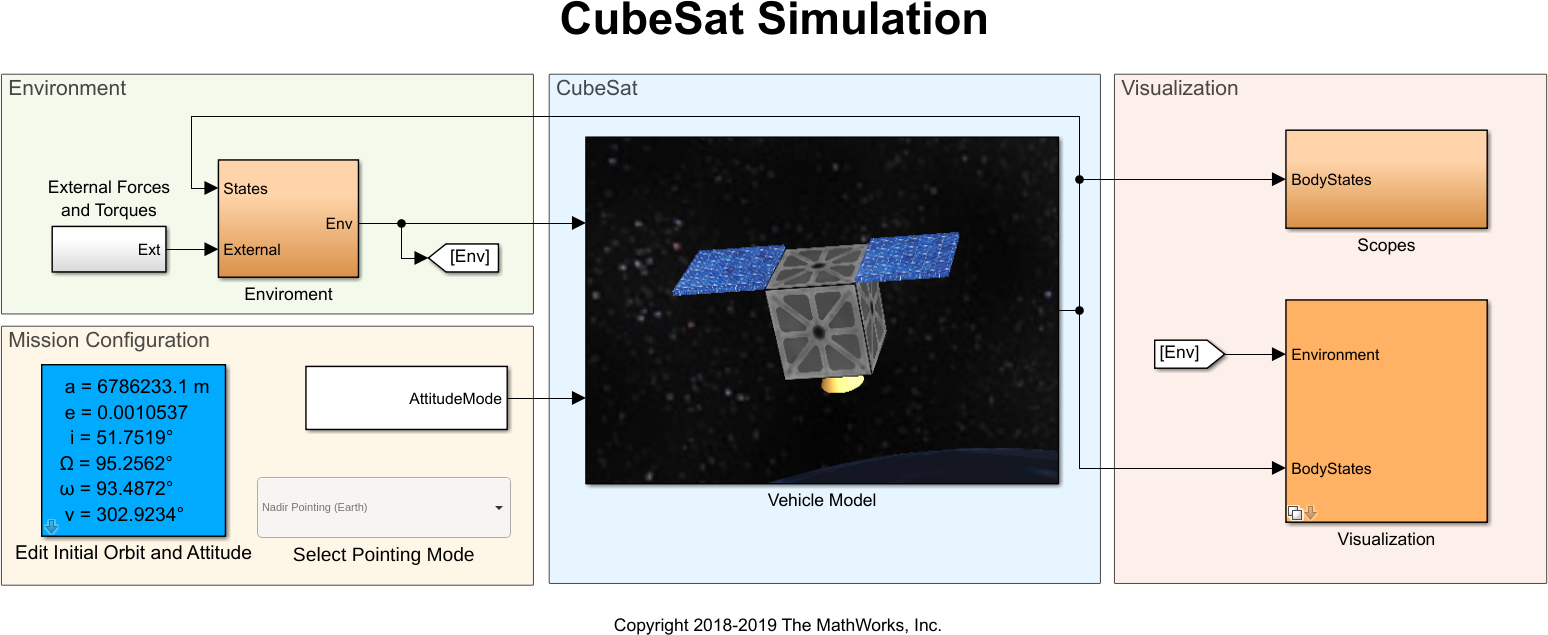
\includegraphics[width=1\textwidth]{1-introduction/matlab_cubesat}
            \caption{Top-level view of the example project of the MATLAB CubeSat Simulation Library}
            \label{fig:matlab_cubesat}
        \end{figure}

        This library, while conceptually most similar to the \ac{tool}, it lacks some functionalities. For example, for actuators, it provides only general models for perfect and second-order actuators. In \ac{tool}, the actuators are full models, which allows not only for reducing the number of layers of abstraction between the user and the simulation, but also for things like calculation of energy expended by the actuator. Also, this toolbox is sparsely documented - while most functionalities are described within their Simulink block masks, there is no comprehensive guide about how to use them in own models \cite{matlabcubesat}.

    \subsubsection{PrincetonSATELLITE Spacecraft Control Toolbox}
        PrincetonSATELLITE Spacecraft Control Toolbox is a commercial solution for building spacecraft Simulations. It contains over two thousand functions for attitude and orbit dynamics, simulation, estimation, analysis and design. This is the most robust and comprehensive toolbox available, includes online API, well written documentation and additional modules for unique applications like formation flying, fusion propulsion or solar sails. This would be the best choice for most use-cases, yet it is a paid solution and even the cheapest option - CubeSat Edition - may be out of price range for smaller teams \cite{princeton}.

    \subsubsection{PROPAT Toolbox}
        PROPAT is is a small set of functions in Matlab to simulate and propagate orbit and attitude of an Earth's satellite, developed by the single person as an open-source toolbox. Several functions allow to transform between orbit and attitude coordinates and for propagation or rigid body attitude. PROPAT contains only MATLAB scripts, which while useful and can be used as a part of the simulation, do not combine into a model of a whole spacecraft's \ac{adcs} subsystem \cite{propat}.

    \subsubsection{GAST Toolbox}
        \begin{figure}[H]
            \centering
            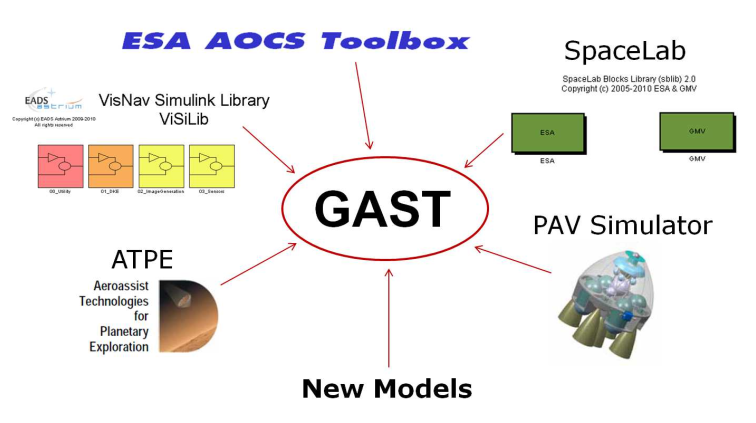
\includegraphics[width=1\textwidth]{1-introduction/gast}
            \caption{Representation of the consolidation of TEC-ECN toolboxes}
            \label{fig:gast}
        \end{figure}

        The GAST toolbox is the result of the consolidation of several toolboxes available in \ac{tec} of \ac{estec}, such as the \ac{aocs} Toolbox, the SpaceLAB library, the ViSiLib library, the ATPE simulator, and the PAV simulator. In addition to consolidating these toolboxes, new models were developed for the GAST toolbox according to the needs of the section. \autoref{fig:gast} shows a pictorial representation of the consolidation of the toolboxes of TEC-ECN. This software was developed in \ac{tec} in 2008, but since it is a product of \ac{esa}, it is not available for use for wider audience \cite{gast}.

    \subsubsection{User-created modules available on MathWorks MATLAB Central}
    As MATLAB is one of the most popular scripting language between engineers, and along with Simulink package it provides tools helpful for simulating mechanical systems, there are many user created modules and packages.
    
    MATLAB Central is a network for asking questions about MATLAB software, discussing solutions and sharing MATLAB and Simulink solutions and files \cite{matlabcentral}. On a subsection called File Exchange there are many files available to use within MATLAB framework, some of them relevant to spacecraft design. The most notable examples are listed below.

        \paragraph*{SAT-LAB}\hspace{0pt}\\
            % \todo[inline]{https://www.mathworks.com/matlabcentral/fileexchange/63344-sat-lab-a-matlab-graphical-user-interface-for-simulating-and-visualizing-keplerian-satellite-orbits}
            SAT-LAB is a MATLAB-based Graphical User Interface (GUI), developed for simulating and visualizing satellite orbits. The primary purpose of SAT-LAB is to provide a software with a user-friendly interface that can be used for both academic and scientific purposes. While a useful tool, it is only suitable for initial mission planning.\cite{satlab}

        \paragraph*{Satellite Orbit Modeling}\hspace{0pt}\\
            % \todo[inline]{https://www.mathworks.com/matlabcentral/fileexchange/54877-satellite-orbit-modeling}
            A collection of MATLAB scripts used for modelling of satellite's perturbed motion with special perturbations approach. While it is very robust, as it can be applied to any problem in celestial mechanics, this module is useful for orbit modeling, not \ac{aocs} system design \cite{som-matlab}.
            
        \paragraph*{Smart Nanosatellite Attitude Propagator (SNAP)}\hspace{0pt}\\
            % todo[inline]{https://www.mathworks.com/matlabcentral/fileexchange/68652-smart-nanosatellite-attitude-propagator-snap}
            The Smart Nanosatellite Attitude Propagator is an attitude propagator for satellites that can be used to analyze the environmental torques affecting a satellite and to design and analyze passive attitude stabilization techniques, such as Passive Magnetic Stabilization, Gravity Gradient Stabilization and Aerodynamic stabilization. This model is the most relevant one for the scope of this thesis, but it lacks possibility to model active attitude stabilization techniques \cite{snap}.

        \paragraph*{Satellite Orbits: Models, Methods and Applications}\hspace{0pt}\\
            % \todo[inline]{https://www.mathworks.com/matlabcentral/fileexchange/54840-satellite-orbits-models-methods-and-applications}
            Rather than spacecraft or orbit model, it is a collection of exercises for book \textit{Satellite Orbits: Models, Methods and Applications}. It is interesting from the educational point and refers at least partially to the problem of control system design - mainly GPS sensor. Yet this is not a toolbox by any means \cite{orbitsaddon}.
        
        \paragraph*{Apollo 11 Moon Landing - 50th Anniversary Model}\hspace{0pt}\\
            % https://www.mathworks.com/matlabcentral/fileexchange/72127-apollo-11-moon-landing-50th-anniversary-model
            This example shows how Richard Gran and the other engineers who worked on the Apollo Lunar Module digital autopilot design team could have done it using Simulink, Stateflow, Aerospace Blockset and Simulink 3D Animation if they had been available in 1961. Although it is a very notable example of how MATLAB software family can be used to simulate a whole mission, to use it for either own spacecraft or educational purposes would require much more reverse engineering and modifications than creating a new model \cite{apollo}. 

% \todo[inline]{Also, write somewhere that while the Toolboxes/Simulations like these are present within papers online, they are nowehere to be found to download and it is hard and time-consuming to recreate them from papers.}
